\begin{surferPage}[Septica heptagonal]{Séptica con simetría heptagonal}
    Esta superficie, parecida a una estrella, tiene grado $7$. 
    Hasta no hace mucho, sus $84$ puntos singulares eran el máximo conocido para sépticas
    con singularidades reales. Recién en el año $2004$, este máximo pasó a ser de $99$, 
    con la contribución de Oliver Labs.
    
    Las tres 'capas' que se pueden ver en la imagen interactiva tienen su origen
    en el uso de polinomios de Tchebichev (como en la óctica de Chmutov).  
    De hecho, se trata de una variante de las superficies de Chmutov, propuesta por Duco van Straten:
    en lugar de la curva plana $T_d(x)+T_d(y)$ se usa la ecuación
    $S_7(x,y)$ del heptágono regular: 
    \[S_7(x,y) + \lambda \cdot T_d(z) = 0,\]
    siendo $\lambda\in\RR$ un valor elegido convenientemente.

  
    \vspace*{-0.3em}
    \begin{center}
      \begin{tabular}{c@{\qquad}c}
        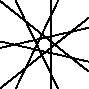
\includegraphics[height=1.5cm]{../../common/images/labsseptic1.pdf}
        &
        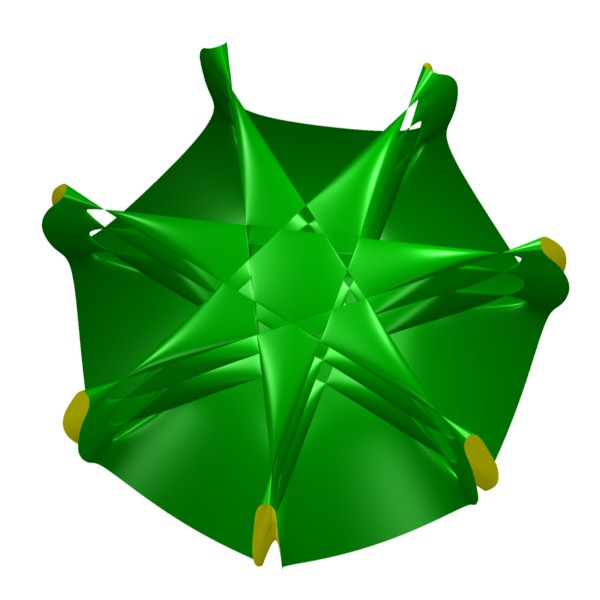
\includegraphics[height=1.5cm]{../../common/images/septic_7eck_von_oben}
      \end{tabular}
    \end{center}
    \vspace*{-0.3em}
\end{surferPage}
